\documentclass[10pt]{beamer} % Определяем тип документа как презентацию
% в квадратных скобках размер шрифта: 8pt, 9, 10, 11 (def), 12, 14, 17, 20.

% Общее:
\usetheme{CambridgeUS} % колонтитулы, углы, и другая красота
% Другие темы можно найти на https://latex-beamer.com/tutorials/beamer-themes/
\usecolortheme{seahorse} % но по факту мы почти все цвета сами задаем
% https://deic.uab.cat/~iblanes/beamer_gallery/index_by_color.html
\usefonttheme{professionalfonts}

\usepackage {mathtools} % красивая математика
\usepackage{amsmath,amsfonts,amssymb,amsthm,mathtools} % еще математика

\usepackage[
backend=biber,
style=numeric,
sorting=nty
]{biblatex} % для библиографии
\addbibresource{references.bib}
\usepackage{hyperref} % для ссылок



% Создаем цвета
\definecolor{darkredNES}{RGB}{115,15,15} % тёмно-красный
\definecolor{darkblueNES}{RGB}{20,20,100} % тёмно-синий
\definecolor{redNES}{RGB}{170,35,35} % красный посветлее
\definecolor{darkgreenNES}{RGB}{7,110,7} % тёмно-зеленый
\definecolor{alertredNES}{RGB}{125,25,25} % красный средний
% Однако в основном проще пользоваться стандартными цветами, подробнее тут:
% https://www.overleaf.com/learn/latex/Using_colours_in_LaTeX

\setbeamercolor*{palette primary}{bg=darkredNES} %правые рамки
\setbeamercolor*{palette secondary}{bg=darkredNES, fg = white} %центральные
\setbeamercolor*{palette tertiary}{bg=darkredNES, fg = white} %левые

\setbeamercolor*{titlelike}{fg=darkredNES} % названия слайдов
\setbeamercolor*{title}{bg=darkredNES, fg = white} % титул и отделы
\setbeamercolor*{item}{fg=redNES} % для списков (например, в оглавлении)
\setbeamercolor*{caption name}{fg=darkblueNES} % названия картинок
\setbeamercolor{alerted text}{fg=alertredNES} % выделенка

\setbeamertemplate{blocks}[rounded, shadow=true]
\setbeamercolor{block title}{bg=darkblueNES, fg=white}
\setbeamercolor{block title alerted}{bg=alertredNES, fg=white}
\setbeamercolor{block title example}{bg=darkgreenNES, fg=white}

\setbeamercolor{bibliography entry author}{fg=black}
\setbeamercolor{bibliography entry title}{fg=black}
\setbeamercolor{bibliography entry note}{fg=darkblueNES}

\setbeamercolor{page number in head/foot}{fg=white}




% Для русского нам пригодится
\usepackage[english,russian]{babel} % локализация и переносы
\usepackage{fontspec}
\usepackage[T1,T2A]{fontenc} % кодировка
\usepackage[utf8]{inputenc} % кодировка исходного текста
\usepackage{cmap} % поиск в PDF
\usepackage{mathtext} % русские буквы в формулах



% Шрифты
% \setsansfont{Times New Roman} % Настройка Шрифта
% \setsansfont{Noto Sans} этот можете использовать, если вам не нравятся засечки на буквах
% \setmainfont{Arial} % Дополнительно
% \setmonofont{Arial} % Нужно Разобраться за что они отвечают
% Другие шрифты можно поскачивать на https://www.ctan.org/tex-archive/fonts


% Работа с картинками
\usepackage{graphicx} % Для вставки рисунков
\setlength\fboxsep{3pt} % Отступ рамки \fbox{} от рисунка
\setlength\fboxrule{1pt} % Толщина линий рамки \fbox{}
\usepackage{wrapfig} % Обтекание рисунков текстом
\DeclareGraphicsExtensions{.pdf,.png,.jpg,.HEIC} % работа с форматами
% \graphicspath{{images/}} % папки с картинками, в оверлифе это не нужно
% Ещё о картинках https://www.overleaf.com/learn/latex/Inserting_Images



% Работа с таблицами
\usepackage{array,tabularx,tabulary,booktabs} % Дополнительное для таблиц
\usepackage{longtable} % Длинные таблицы
\usepackage{multirow} % Слияние строк в таблице



% Свои команды, если лень прописывать \mathbb итп.
\def\E{\exists} % существует
\def\A{\forall} % для всех

\def\La{\mathcal{L}} % калиграфическое L (Лагранжиан, преобразования Лапласа)
\def\la{\lambda} % лямбда
\def\a{\alpha} % альфа
\def\b{\beta} % бэта
\def\e{\varepsilon} % эпсилон (покрасивее)
\let\phi\varphi % фи (покрасивее)

\def\N{\mathbb{N}} % натуральные
\def\Z{\ensuremath{\mathbb{Z}}} % целые
\def\R{\mathbb{R}} % рациональные
\def\C{\mathbb{C}} % комплексные

\def\~{\sim} % подобно



%Возможно, у вас возникнут проблемы с буквой @, попробуйте одно из следующих:
%\makeatletter
%\makeatother 
% В преамбуле можно сделать небольшие изменения (цвет, шрифт итд.) Если есть желание изменить больше, возможно, проще выбрать другой шаблон.

% Начнем работу с презентацией
\usepackage{comment}
\usepackage{listings}
\usepackage[export]{adjustbox}
\usepackage{graphicx}
\graphicspath{ {./images/} }
\usepackage{csquotes}
%Для начала подготовим титульный лист и оглавление
%Логотип РЭШ
% \titlegraphic{\includegraphics[height=1.5cm]{logo.jpg}}

%Размеры шрифтов титульного листа; Цвета определены в преамбуле
\setbeamerfont{title}{size=\huge}
\setbeamerfont{subtitle}{size=\large}
\setbeamerfont{author}{size=\normalsize}
\setbeamerfont{date}{size=\normalsize}
\setbeamerfont{institute}{size=\normalsize}
% Больше о шрифтах вы найдете в том числе по следующей ссылке:
% https://tex.stackexchange.com/questions/183052/what-are-all-the-possible-first-arguments-to-setbeamerfont

%Тут квадратные скобки --- всё, что будет внизу странички
\title[ФПМИ МФТИ]{Оптимизация экономического портфеля с использованием методов машинного обучения}
\subtitle{Бакалаврский диплом}
\author[Михаил Давыдов]{Михаил Давыдов}
\institute[]{ФПМИ МФТИ, кафедра дискретной математики}
\date[\textcolor{white}{\today}]{\today}



% Следующее пригодится, если нужно показывать начало секции с оглавлением
%\AtBeginSection[]
%{
%  \begin{frame}
%    \frametitle{Contents}
%    \tableofcontents[currentsection]
%  \end{frame}
%}

\AtBeginSection[]{
  \begin{frame}
  \vfill
  \centering
  \begin{beamercolorbox}[sep=8pt,center,shadow=true,rounded=true]{title}
    \usebeamerfont{title}\insertsectionhead\par%
  \end{beamercolorbox}
  \vfill
  \end{frame}
}



\begin{document} % начнем саму презентацию
\setsansfont{Noto Sans} % этот можете использовать, если вам не нравятся засечки на буквах
\newcounter{currentenumi}
\lstset{escapeinside={@(}{)@}}

\frame{\titlepage} % сделаем титульный слайд и оглавление:

% Далее начнем работу со слайдами:
\begin{frame}{Введение}
    Инвесторы вкладывают свои деньги в акции, и хотят использовать для распределения денег эффективные алгоритмы. \pause
    Если инвестор изначально не обладает информацией о стоимости активов, то в качестве модели можно использовать модель многоруких бандитов
    \begin{itemize}
        \item<3-> Есть $n$ рычагов, $i$-ый рычаг соответствует какому-то распределению со средним $m_i$. Изначально распределения, как и средние, неизвестны.
        \item<4-> При нажатии на $i$-ый рычаг выдается награда в соответствии с $i$-ым распределением.
        \item<5-> Задача -- найти $\underset{\textbf{p} \in \Delta^n}{\arg \max} \: \textbf{p}^T \cdot \textbf{m} = \sum_{i=1}^n p_i m_i$, где $\Delta^n = \left\{ \textbf{p} = (p_1, ..., p_n) : \left(\sum_{i=1}^n p_i = 1\right) \wedge (\forall i \; p_i \geqslant 0) \right\}$, $\textbf{p}$ отвечает за долю от общих средств, вкладываемых в каждый актив на каждом шаге.
        \item<6-> Равносильно нахождению рычага с наибольшим средним
    \end{itemize}
\end{frame}
\begin{frame}{Учет рисков}
    \begin{itemize}
        \item<1-> Появляется дисперсия $\sigma_i^2$.
        \item<2-> Задача -- найти \[\underset{\textbf{p} \in \Delta^n}{\arg \max} \:
        \left(\textbf{p}^T \cdot \textbf{m} - \lambda \left(\textbf{p}^T\right)^2 \cdot \boldsymbol{\sigma}^2 \right)
        = \sum_{i=1}^n p_i m_i - \lambda \sum_{i=1}^n p_i^2 \sigma_i^2\]
        где $\lambda > 0$ -- коэффициент отвращения, или неприятия к риску.
        \item<3-> В этой трактовке задачи вектор вероятностей может не сосредотачиваться в одном рычаге.
    \end{itemize}
\end{frame}

\begin{frame}{Задачи}
    \begin{enumerate}
        \item<1-> Проанализировать известные подходы в классической задаче о многоруких бандитах на предмет применимости для распределений, отличных от нормального.
        \item<2-> Придумать алгоритмы и подходы для решения задачи о многоруких бандитах с учетом степени отвращения к риску.
        \item<3-> Протестировать созданные подходы на степенных распределениях.
        \item<4-> Оценить степень применимости оценки риска через дисперсию
    \end{enumerate}
\end{frame}

\begin{frame}{Алгоритмы}
    \begin{enumerate}
        \item<1-> Greedy и $\epsilon$-greedy
            $$A_t = \begin{cases}
        \underset{a}{\arg \max} \; Q_t(a), & \text{with probability} \; 1 - \epsilon, \\
        \text{a random action}, & \text{with probability} \; \epsilon.
        \end{cases}$$ 
        \item<2-> Стратегия с позитивной инициализацией ($\forall a \; Q_t(a) = d, \; d > 0$)
        \item<3-> Upper-Confidence Bound selection $$A_t = \underset{a}{\arg \max} \; \left[ Q_t(a) + c \sqrt{\frac{ln \; t}{N_t(a)}} \right], \; c > 0$$
        \item<4-> Gradient bandit
    \end{enumerate}
    \onslide<5->{В конце все алгоритмы были сравнены в зависимости от их гиперпараметров}
\end{frame}

\begin{frame}{Параметры}
    \begin{itemize}
        \item Стандартное нормальное ( $N (0,1)$ или $t_{\infty}$)
        \item Распределение Стьюдента с дисперсией 1 и 3-мя степенями свободы $t_3$ (для единичной дисперсии распределение было домножено на $\sqrt{\frac{1}{3}}$)
        \item Распределение Стьюдента нормированное $t_{2.1}$ с $2.1$ степенями свободы.
        \item Распределение Стьюдента с 2-мя степенями свободы $t_2$
        \item Распределение Коши $t_1$ (только в задаче без учета риска)
    \end{itemize}
\end{frame}

\begin{frame}{Результаты -- $\epsilon$-greedy}
    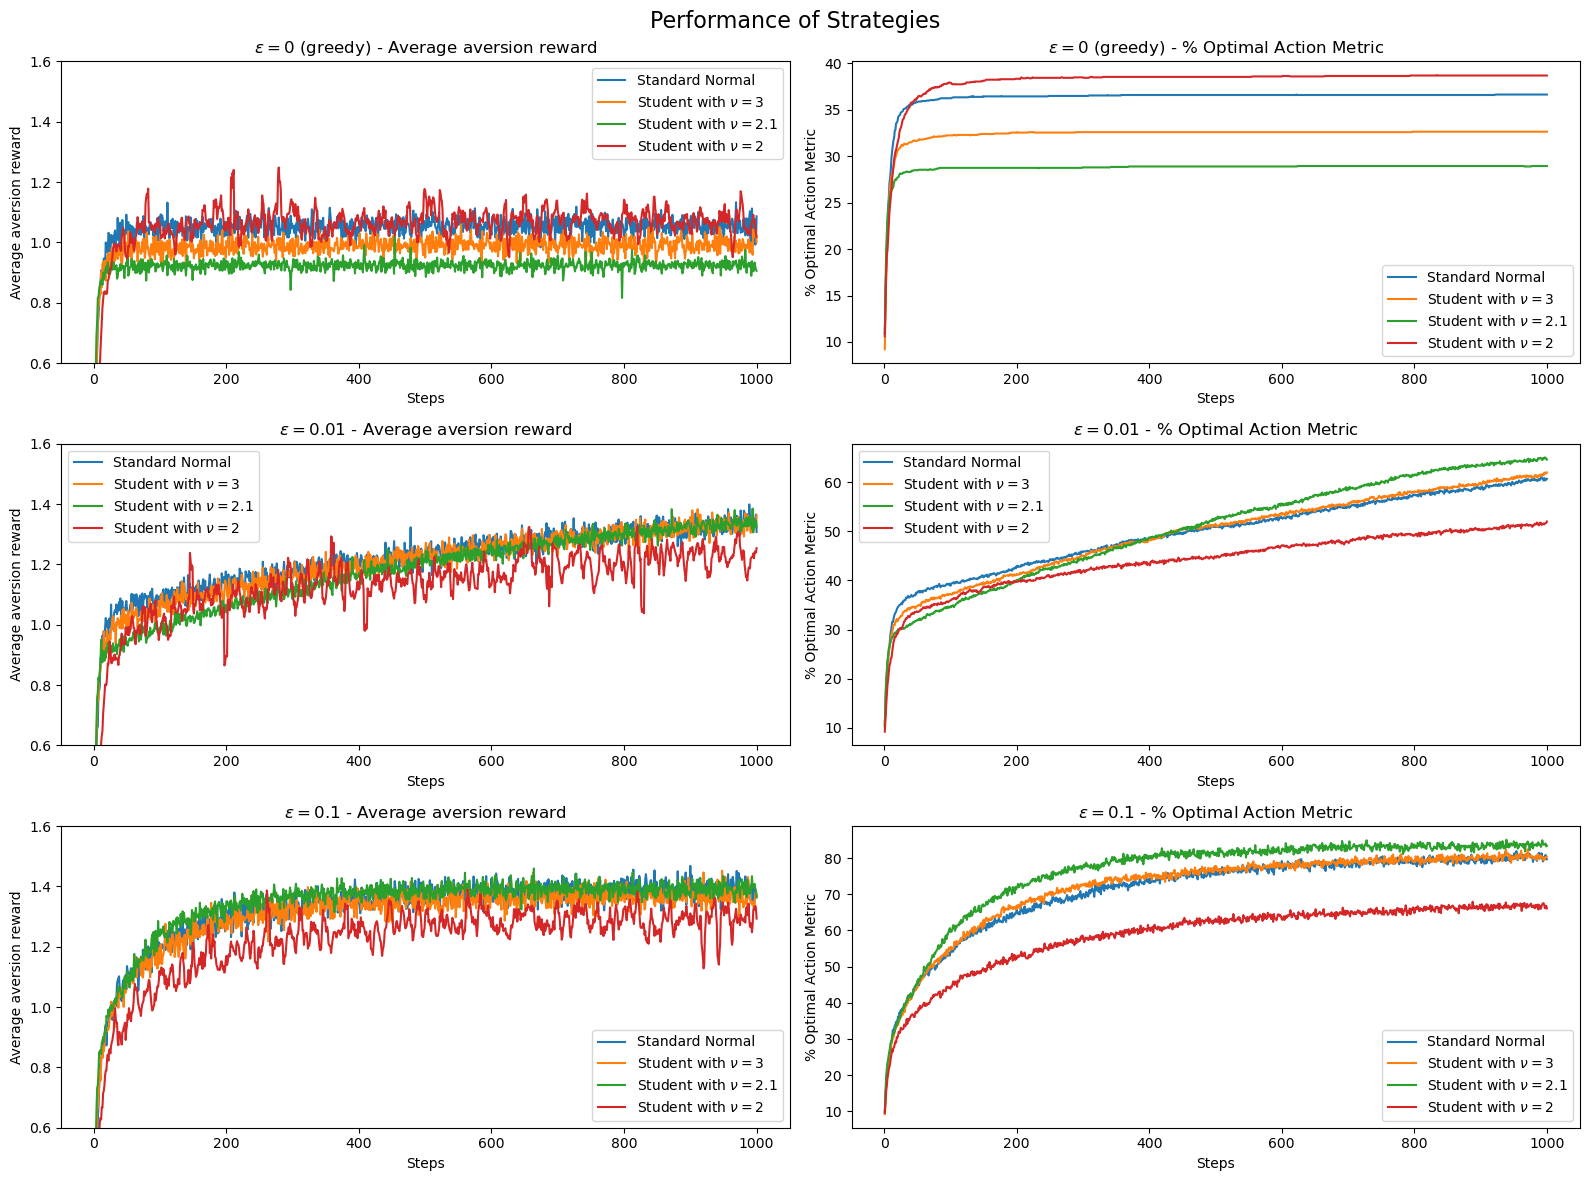
\includegraphics[scale=0.2,center]{images/experiments_classic/eps_greedy/second.png}
\end{frame}
\begin{frame}{Результаты -- финальное тестирование}
    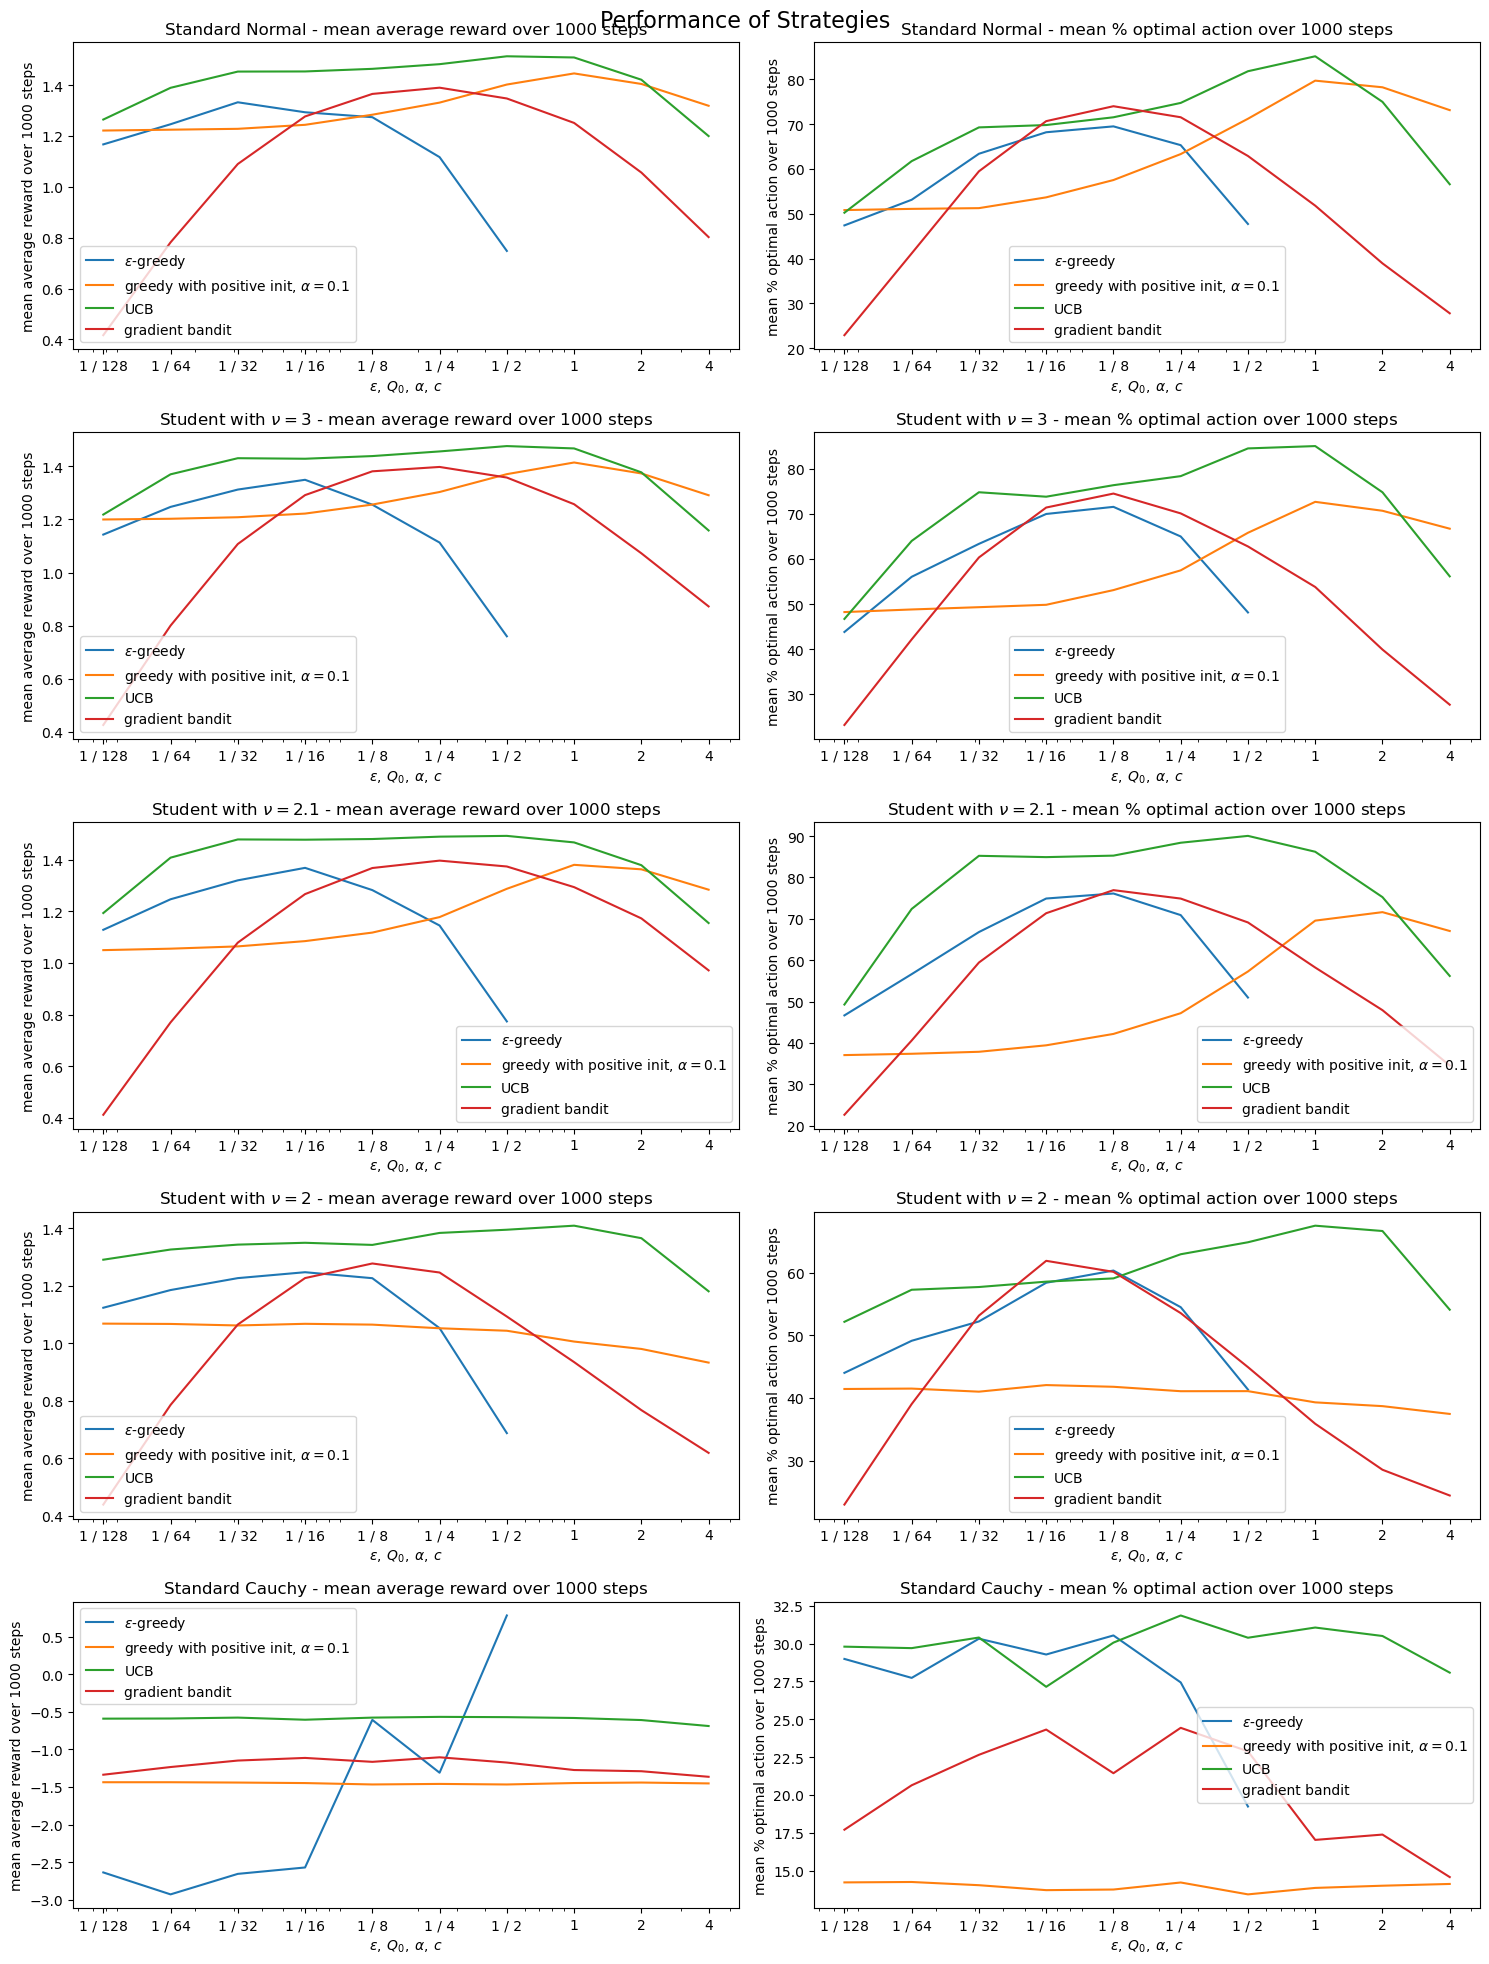
\includegraphics[scale=0.15,center]{images/experiments_classic/overall/overall.png}
\end{frame}
\begin{frame}{Выводы}
    Проделанные эксперименты позволяют судить о том, что Gradient bandits, $\epsilon$-greedy и UCB -- стратегии показывают высокую эффективность на степенных распределениях. UCB при этом лучшая из стратегий.
\end{frame}


\begin{frame}{Результаты}
    \begin{enumerate}
        \item <1-> Разработаны градиентный жадный и алгоритмический жадный алгоритмы для вычисления \[\underset{\textbf{p} \in \Delta^n}{\arg \max} \:
        = \sum_{i=1}^n p_i m_i - \lambda \sum_{i=1}^n p_i^2 \sigma_i^2\], при известных $m_i$ и $\sigma_i^2$, причем последний работает за $O(n \log n)$
        \item <2-> Адаптированы стратегии $\epsilon$-greedy, adaptive $\epsilon$, positive initialization, UCB, gradient bandits.
        \item <3-> Создана стратегия с корректировкой дисперсии, переработана стратегия VDBE.
    \end{enumerate}
\end{frame}

\begin{frame}{Метрики}
    \begin{itemize}
        \item <1-> Среднее сожаление: чем ближе к 0, тем лучше. Если $< 0$, то алгоритм ``переоценивает'' себя.
        \item <2-> Среднее реальное сожаление: всегда $\geq 0$, чем ниже, тем лучше.
        \item <3-> Процент оптимальных действий (чем выше, тем лучше): $$\delta = 1 - \frac{1}{2}\sum_{i=1}^n |p_i - p_{i, max}|$$
    \end{itemize}
\end{frame}
\begin{frame}{Результаты -- $\epsilon$-greedy}
    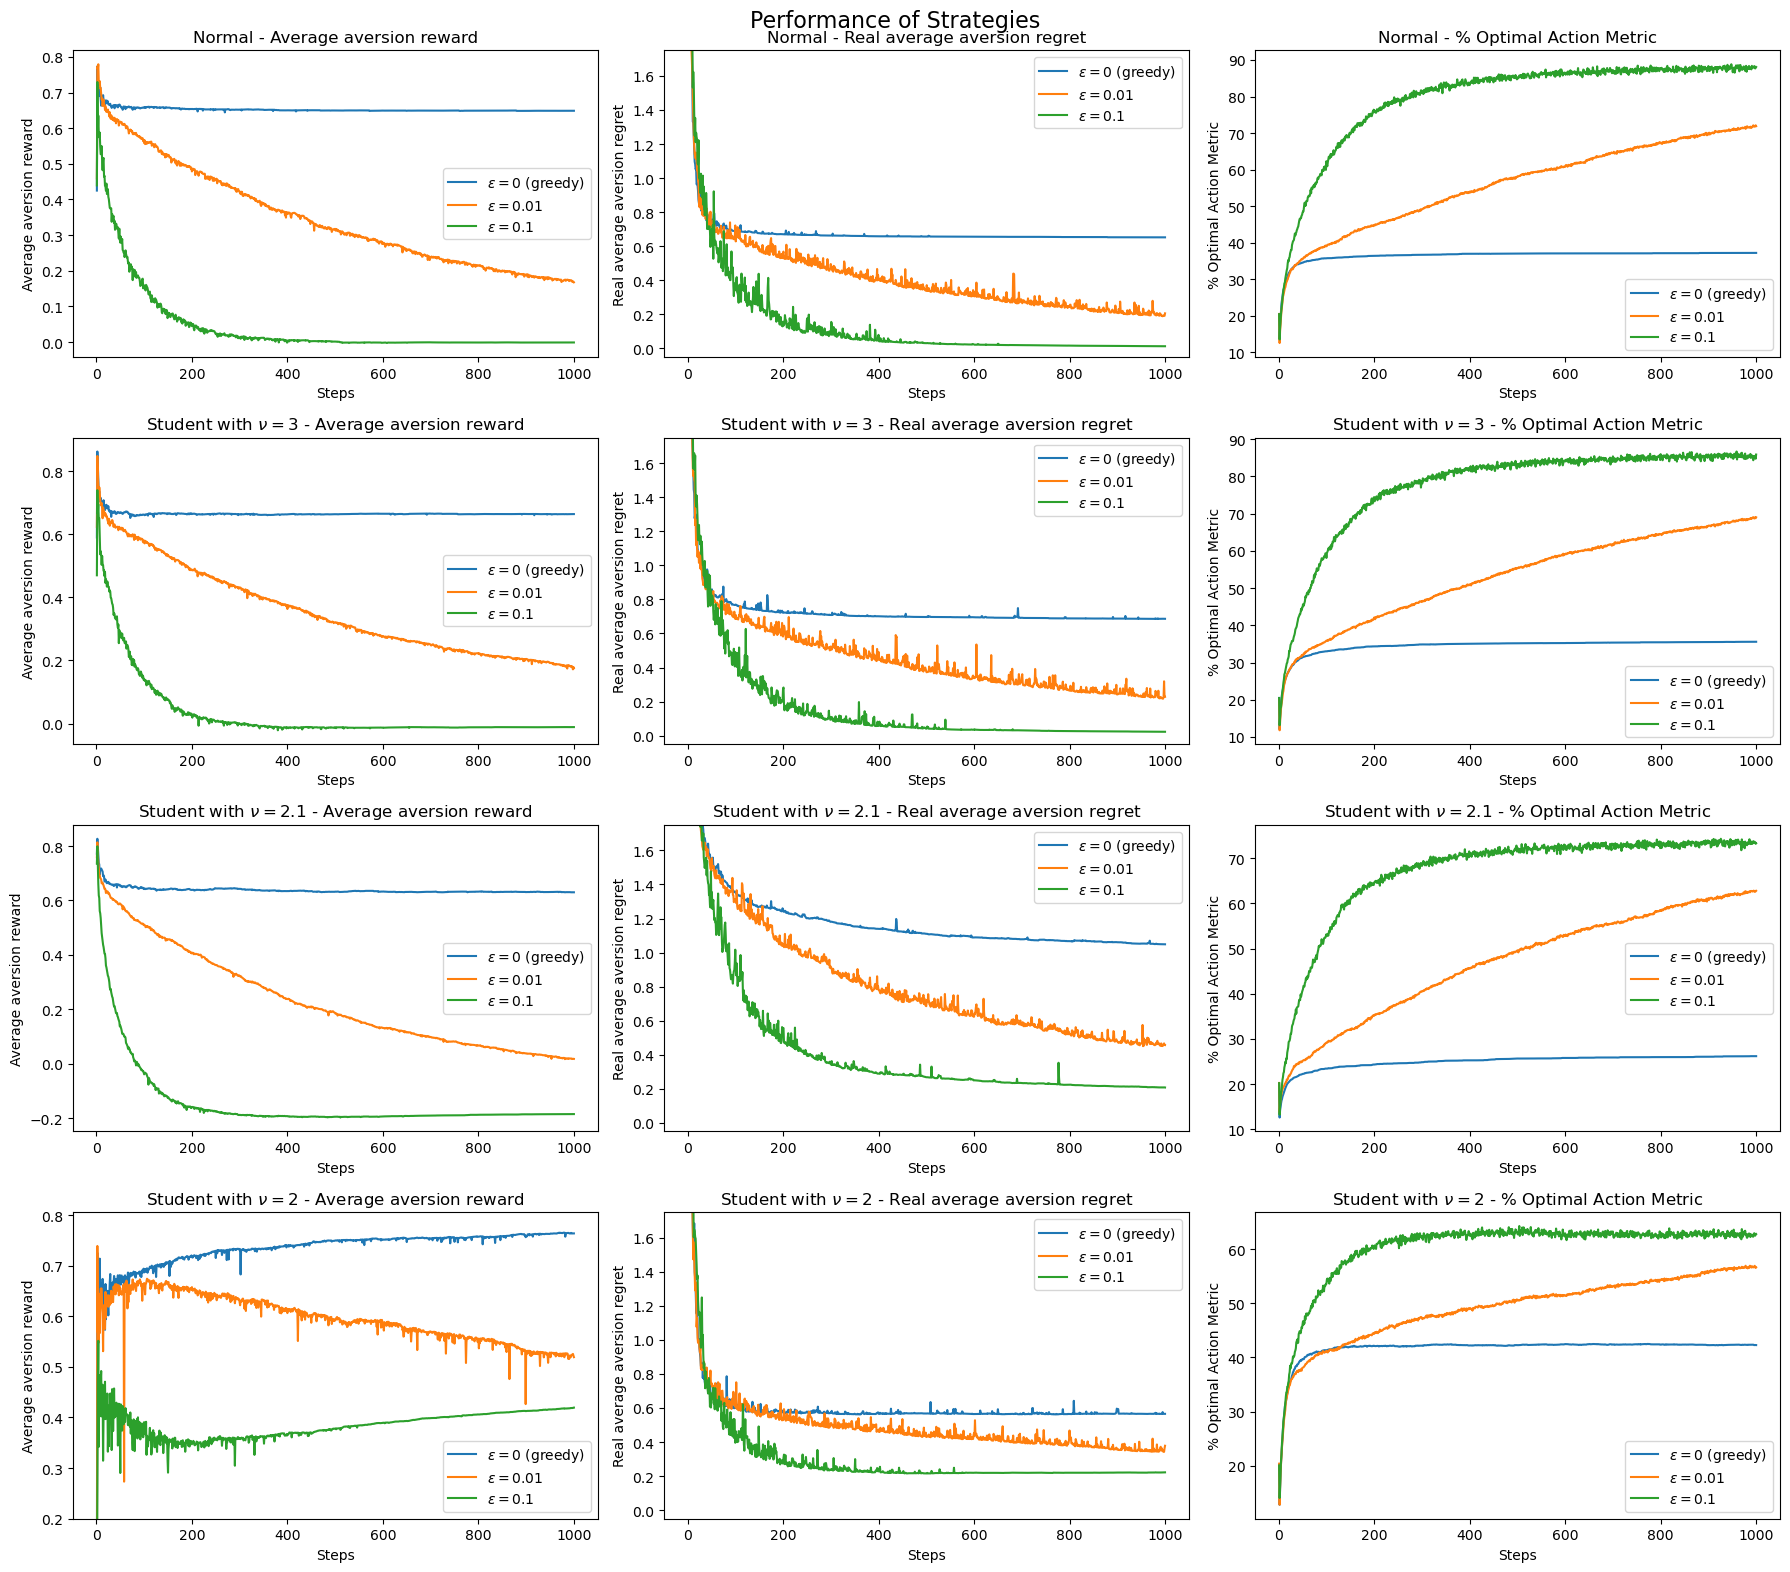
\includegraphics[scale=0.17,center]{images/experiments_aversion/eps_greedy/compare_strategies_inner.png}
\end{frame}
\begin{frame}{Результаты -- $\epsilon$-greedy}
    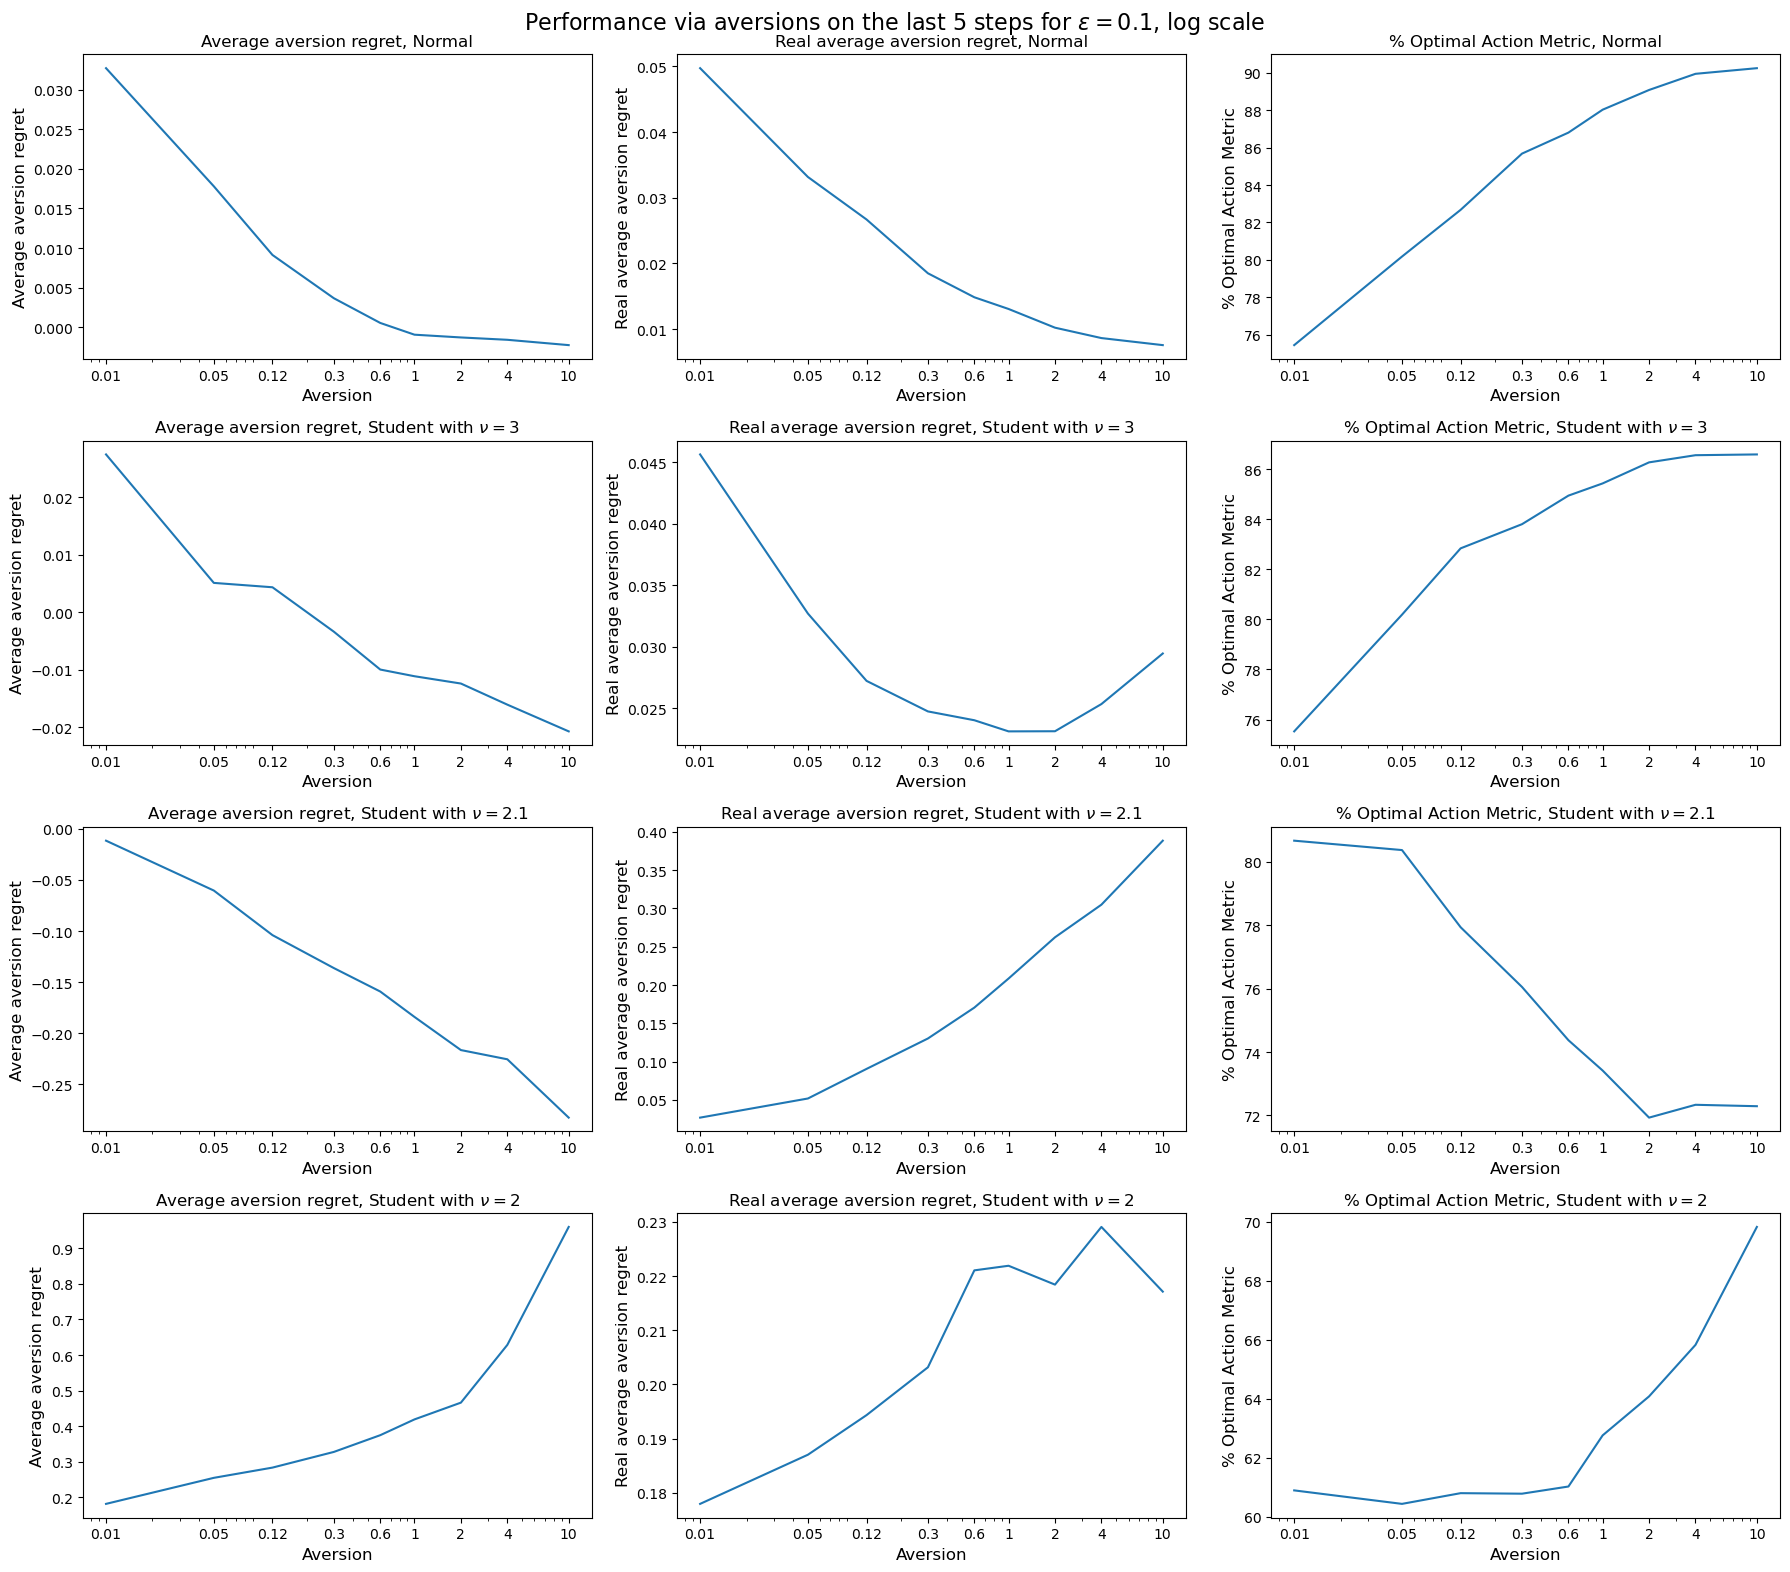
\includegraphics[scale=0.17,center]{images/experiments_aversion/eps_greedy/last_5_steps_outer.png}
\end{frame}
\begin{frame}{Результаты -- Причины плохих метрик для $t_{2.1}$}
    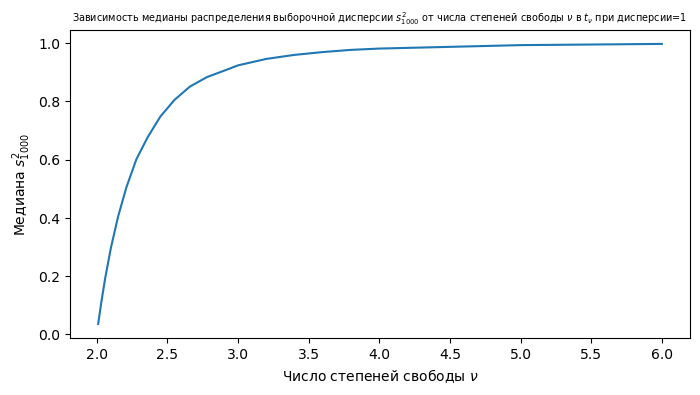
\includegraphics[scale=0.35,left]{images/experiments_aversion/why_2_p_1_so_bad/dependence_median_to_df.png}
    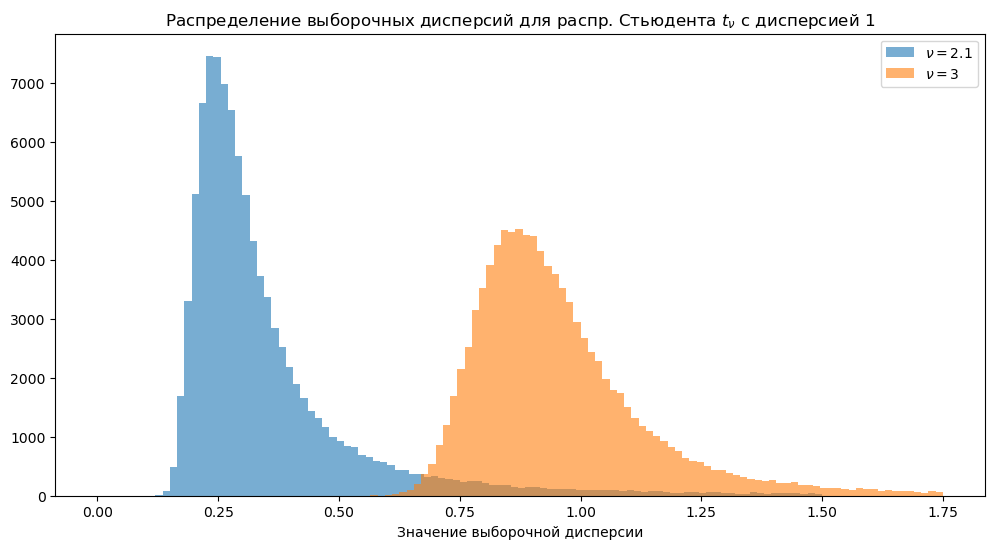
\includegraphics[scale=0.25,right]{images/experiments_aversion/why_2_p_1_so_bad/distribution_of_sample_vars.png}
\end{frame}
\begin{frame}{Результаты -- Коррекция выборочной дисперсии}
    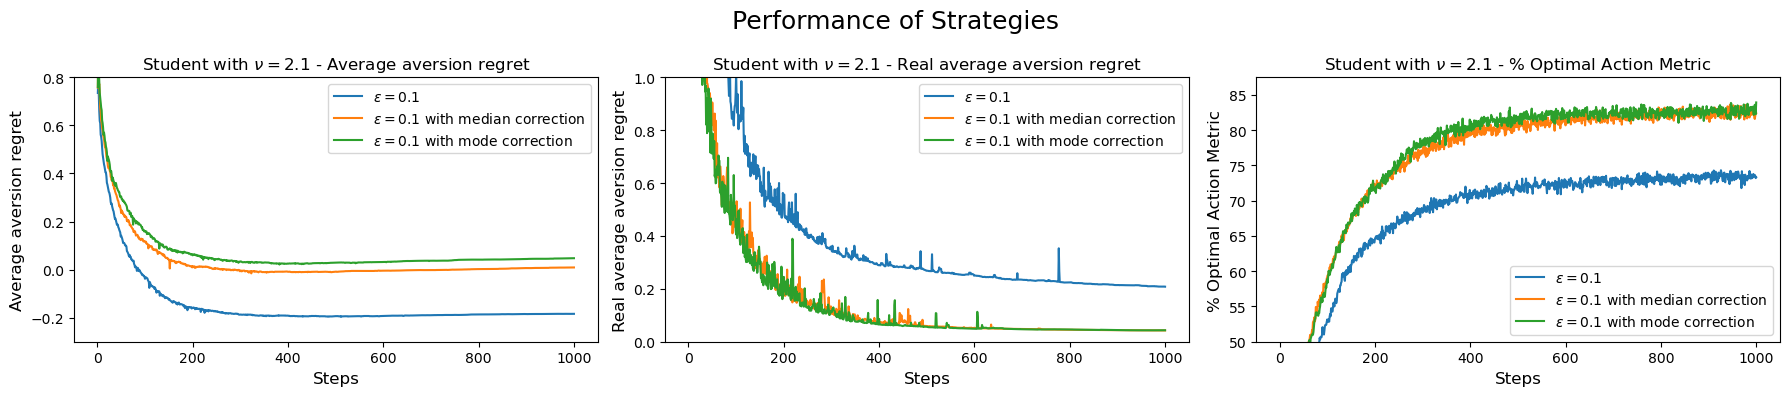
\includegraphics[scale=0.25,center]{images/experiments_aversion/correction/compare_outer.png}
    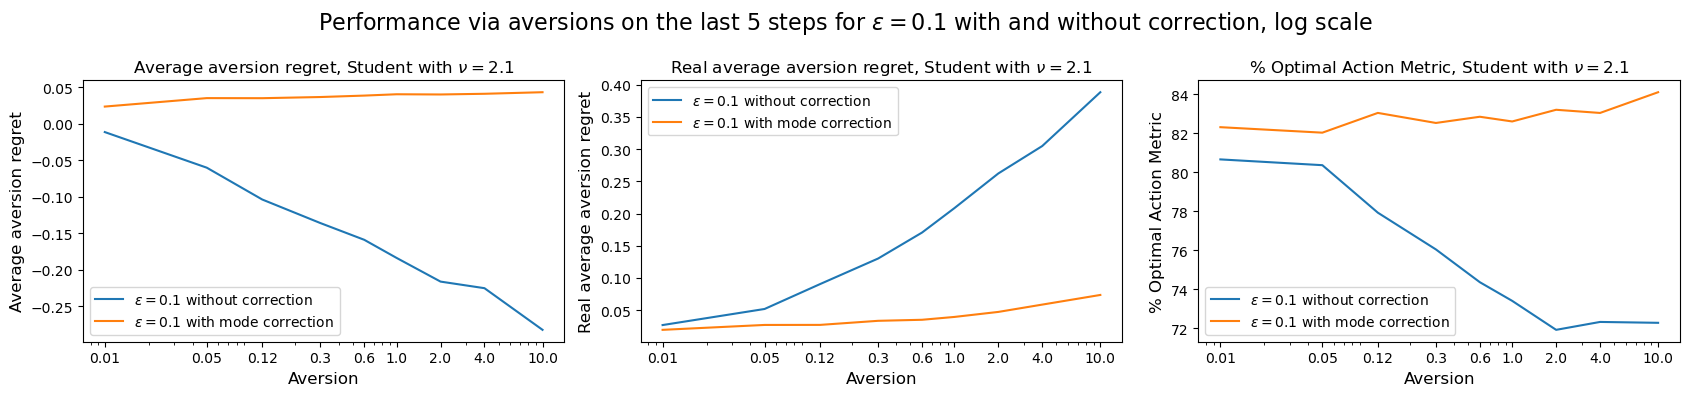
\includegraphics[scale=0.25,center]{images/experiments_aversion/correction/last_5_steps.png}
\end{frame}
\begin{frame}{Жадная позитивная инициализация}
    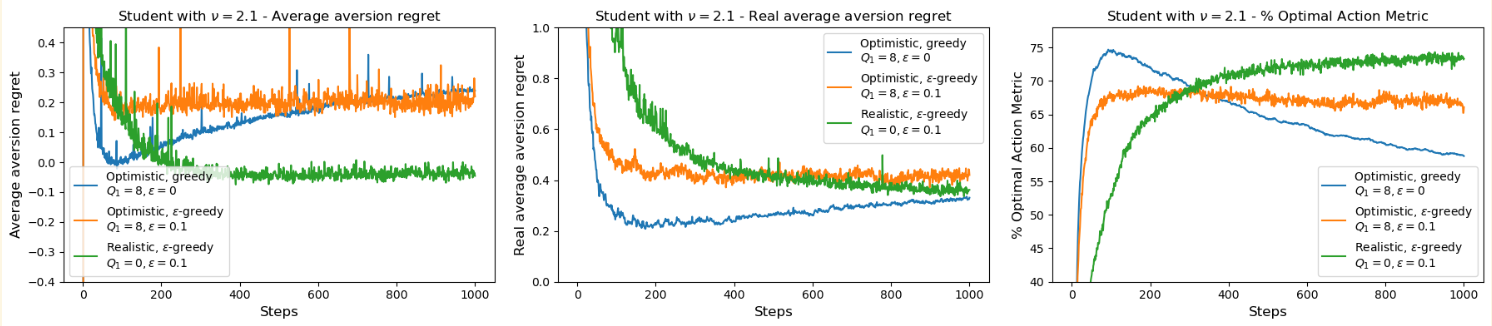
\includegraphics[scale=0.28,center]{images/experiments_aversion/greedy.png}
\end{frame}
\begin{frame}{Результаты -- UCB и gradient bandits}
    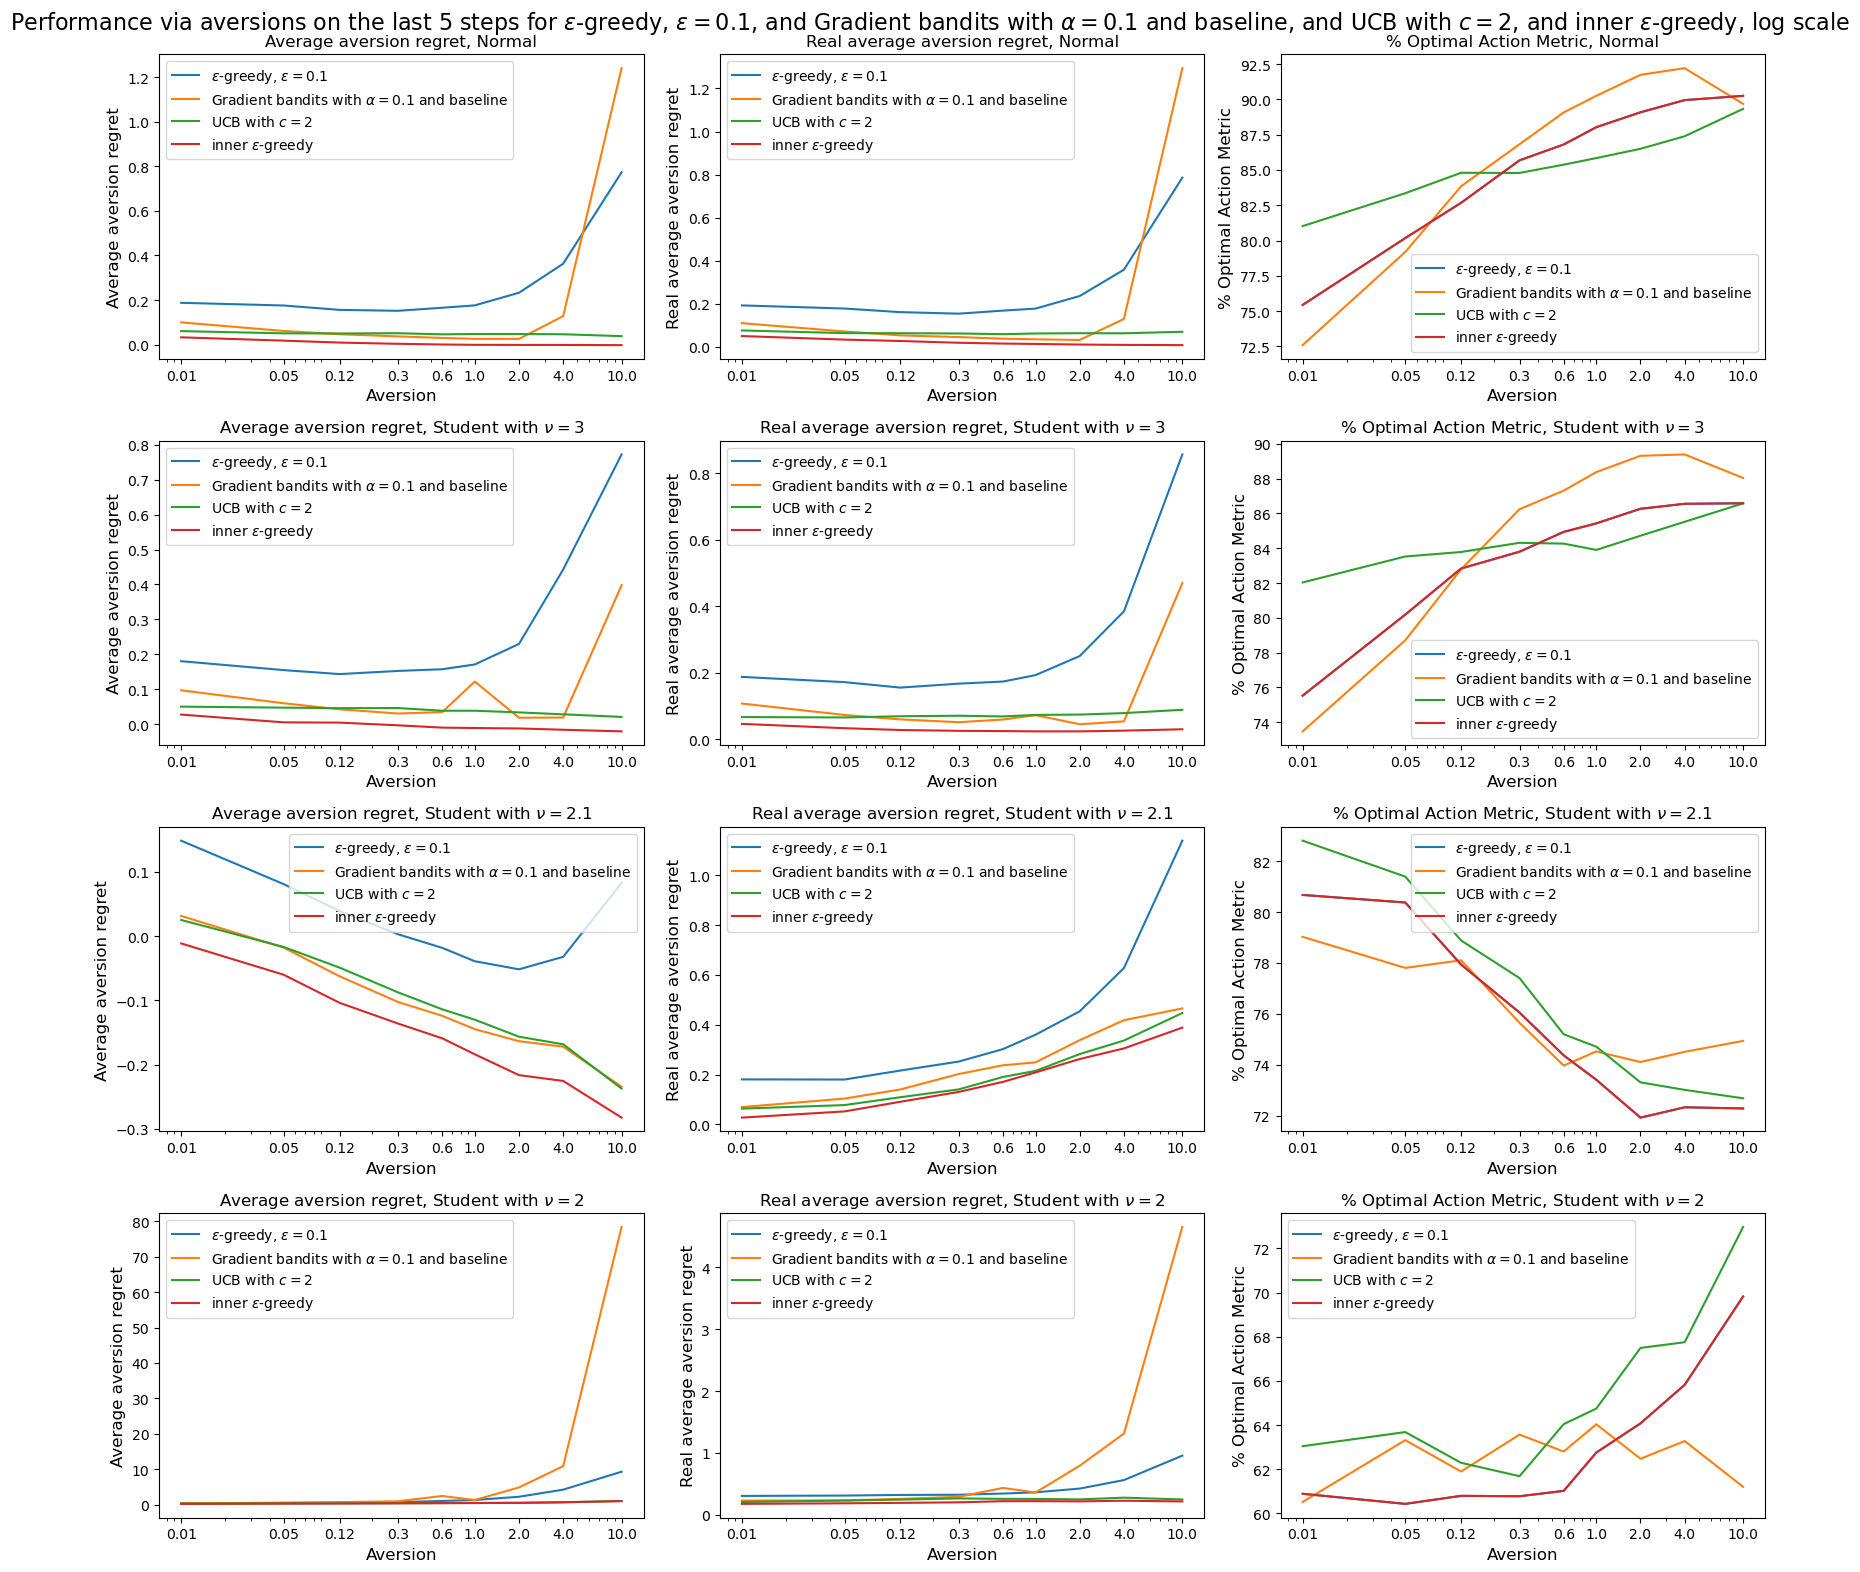
\includegraphics[scale=0.19,center]{images/overall.png}
\end{frame}
\begin{frame}{Выводы}
    \begin{itemize}
        \item<1-> $\epsilon$-greedy дает высокую эффективность для $t_3$ и $t_{\infty}$
        \item<2-> Для улучшения метрик для $t_{2.1}$ можно использовать коррекцию дисперсии.
        \item <3-> UCB даже без замены дисперсии устраняет разрыв между внутренней и внешней вероятностями в $\epsilon$-greedy
        \item <4-> Gradient bandits показывают хорошие результаты и могут быть использованы при больших $\lambda$
        \item <5-> Оценка рисков через дисперсию при $\nu$, близких к 2, слабоприменима
    \end{itemize}
\end{frame}

\begin{frame}{Заключение}
    В результате написания работы:
    \begin{itemize}
        \item<1-> Проанализированы известные подходы в классической задаче о многоруких бандитах на предмет применимости для распределений, отличных от нормального. По результатам UCB показывает себя лучше других алгоритов на всех распределениях.
        \item<2-> Придуманы и адаптированы алгоритмы и подходы для решения задачи о многоруких бандитах с учетом степени отвращения к риску. Среди них: жадный алгоритм за $O(n \log n)$, жадный алгоритм через градиентный подъем, $\epsilon$-greedy, UCB, gradient bandits.
        \item<3-> Протестированы созданные подходы на различных распределениях, получена высокая эффективность стратегий на распределениях Стьюдента с $\nu \geq 3$. Сделан вывод о слабой применимости оценки риска через дисперсию при $\nu$, близких к 2.
    \end{itemize}
\end{frame}

\end{document}
